

\tikzset{every picture/.style={line width=0.3pt}} %set default line width to 0.75pt        

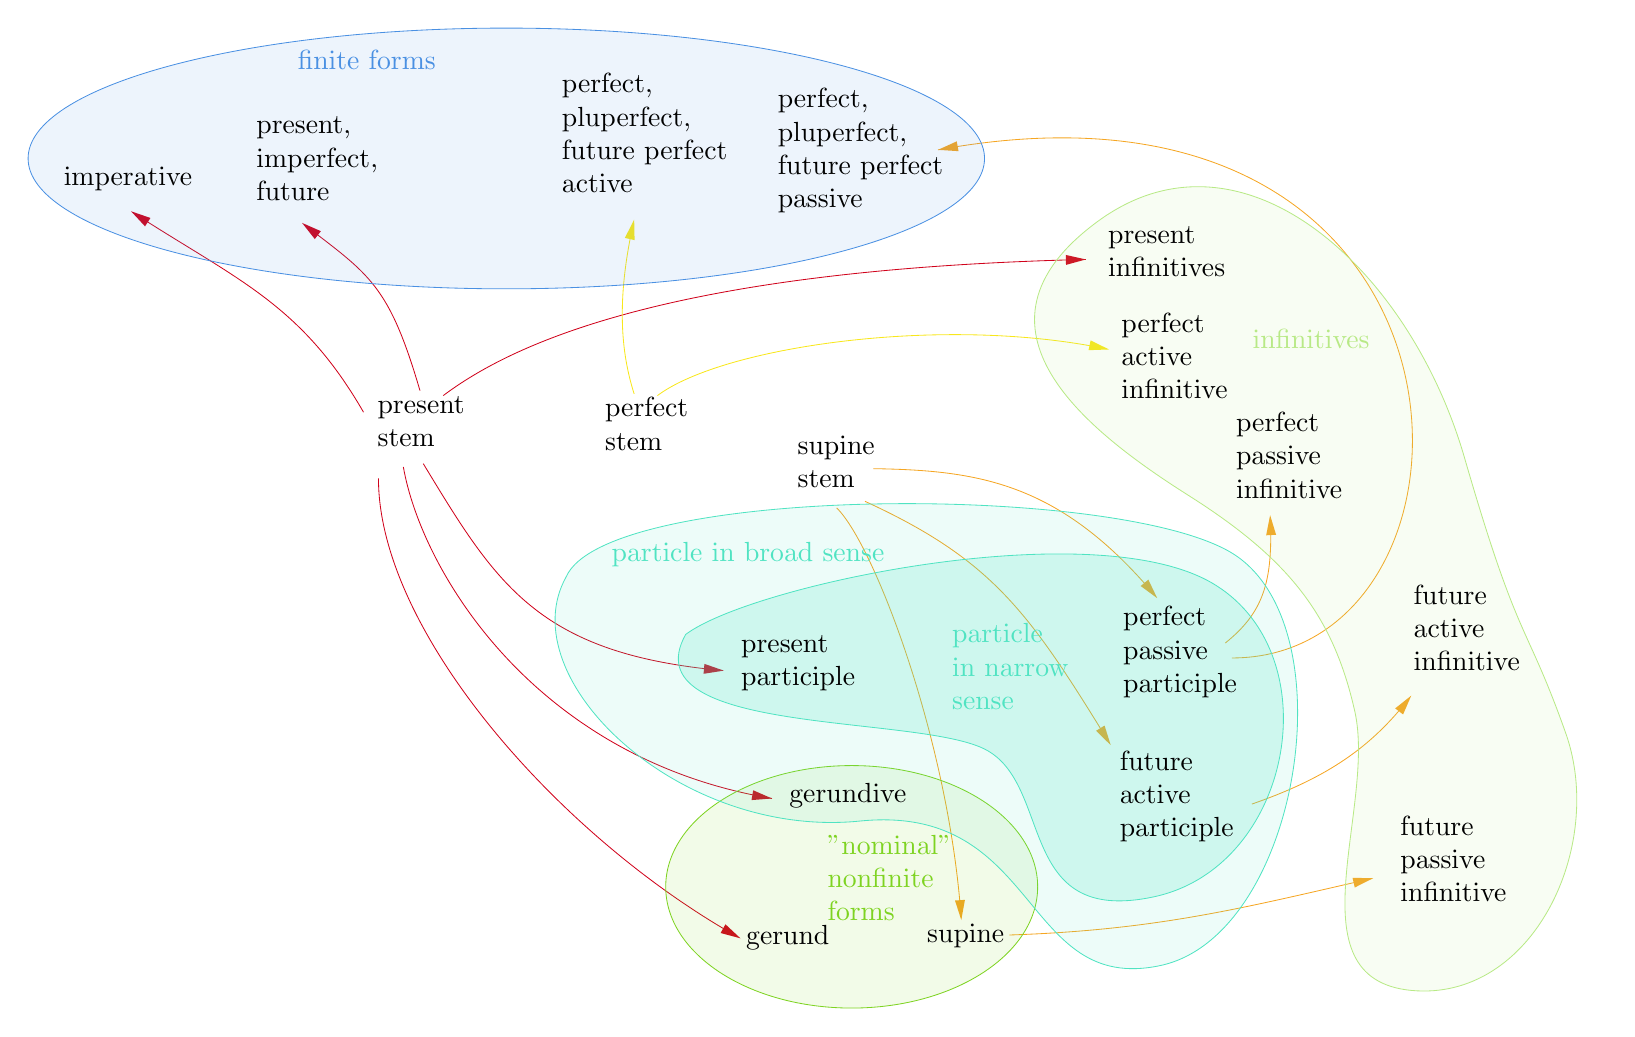
\begin{tikzpicture}[x=0.75pt,y=0.75pt,yscale=-0.8,xscale=0.8]
%uncomment if require: \path (0,697); %set diagram left start at 0, and has height of 697

%Curve Lines [id:da8600925548352094] 
\draw [color={rgb, 255:red, 208; green, 2; blue, 27 }  ,draw opacity=1 ]   (289.01,269.33) .. controls (329.01,239.33) and (422.01,193.33) .. (676.01,187.33) ;
\draw [shift={(676.01,187.33)}, rotate = 178.65] [fill={rgb, 255:red, 208; green, 2; blue, 27 }  ,fill opacity=1 ][line width=0.08]  [draw opacity=0] (12,-3) -- (0,0) -- (12,3) -- cycle    ;
%Curve Lines [id:da7478415205524331] 
\draw [color={rgb, 255:red, 208; green, 2; blue, 27 }  ,draw opacity=1 ]   (275.01,266.33) .. controls (256.2,201.98) and (244.25,196.43) .. (205.2,166.25) ;
\draw [shift={(204.01,165.33)}, rotate = 37.78] [fill={rgb, 255:red, 208; green, 2; blue, 27 }  ,fill opacity=1 ][line width=0.08]  [draw opacity=0] (12,-3) -- (0,0) -- (12,3) -- cycle    ;
%Curve Lines [id:da22329313492102099] 
\draw [color={rgb, 255:red, 208; green, 2; blue, 27 }  ,draw opacity=1 ]   (241.01,279.33) .. controls (203.2,213.66) and (164.4,199.47) .. (101.95,158.94) ;
\draw [shift={(101.01,158.33)}, rotate = 33.06] [fill={rgb, 255:red, 208; green, 2; blue, 27 }  ,fill opacity=1 ][line width=0.08]  [draw opacity=0] (12,-3) -- (0,0) -- (12,3) -- cycle    ;
%Curve Lines [id:da9720425555739067] 
\draw [color={rgb, 255:red, 208; green, 2; blue, 27 }  ,draw opacity=1 ]   (250.01,319.22) .. controls (250.01,411.38) and (358.91,534.94) .. (466.39,595.28) ;
\draw [shift={(468.01,596.18)}, rotate = 209.05] [fill={rgb, 255:red, 208; green, 2; blue, 27 }  ,fill opacity=1 ][line width=0.08]  [draw opacity=0] (12,-3) -- (0,0) -- (12,3) -- cycle    ;
%Curve Lines [id:da9116874614549022] 
\draw [color={rgb, 255:red, 208; green, 2; blue, 27 }  ,draw opacity=1 ]   (265.01,312.33) .. controls (276.01,374.96) and (344.01,487.96) .. (487.01,511.96) ;
\draw [shift={(487.01,511.96)}, rotate = 189.53] [fill={rgb, 255:red, 208; green, 2; blue, 27 }  ,fill opacity=1 ][line width=0.08]  [draw opacity=0] (12,-3) -- (0,0) -- (12,3) -- cycle    ;
%Curve Lines [id:da9399420006349646] 
\draw [color={rgb, 255:red, 208; green, 2; blue, 27 }  ,draw opacity=1 ]   (277.01,310.33) .. controls (320.79,382.6) and (345.76,424.54) .. (456.34,434.81) ;
\draw [shift={(458.01,434.96)}, rotate = 185.1] [fill={rgb, 255:red, 208; green, 2; blue, 27 }  ,fill opacity=1 ][line width=0.08]  [draw opacity=0] (12,-3) -- (0,0) -- (12,3) -- cycle    ;
%Curve Lines [id:da863359914759456] 
\draw [color={rgb, 255:red, 248; green, 231; blue, 28 }  ,draw opacity=1 ]   (404.01,268.33) .. controls (396.09,243.58) and (393.07,211.97) .. (403.69,164.76) ;
\draw [shift={(404.01,163.33)}, rotate = 102.91] [fill={rgb, 255:red, 248; green, 231; blue, 28 }  ,fill opacity=1 ][line width=0.08]  [draw opacity=0] (12,-3) -- (0,0) -- (12,3) -- cycle    ;
%Curve Lines [id:da44942461080998] 
\draw [color={rgb, 255:red, 248; green, 231; blue, 28 }  ,draw opacity=1 ]   (418.01,269.33) .. controls (457.81,239.48) and (590.67,220.74) .. (688.54,241.24) ;
\draw [shift={(690.01,241.55)}, rotate = 192.09] [fill={rgb, 255:red, 248; green, 231; blue, 28 }  ,fill opacity=1 ][line width=0.08]  [draw opacity=0] (12,-3) -- (0,0) -- (12,3) -- cycle    ;
%Curve Lines [id:da6857007576480554] 
\draw [color={rgb, 255:red, 245; green, 166; blue, 35 }  ,draw opacity=1 ]   (543.01,333) .. controls (619.63,368.19) and (641.79,399.53) .. (690.28,478.65) ;
\draw [shift={(691.01,479.85)}, rotate = 238.51] [fill={rgb, 255:red, 245; green, 166; blue, 35 }  ,fill opacity=1 ][line width=0.08]  [draw opacity=0] (12,-3) -- (0,0) -- (12,3) -- cycle    ;
%Curve Lines [id:da10519824034130609] 
\draw [color={rgb, 255:red, 245; green, 166; blue, 35 }  ,draw opacity=1 ]   (548.01,313.33) .. controls (610.7,314.32) and (660.51,321.26) .. (718.14,390.28) ;
\draw [shift={(719.01,391.33)}, rotate = 230.36] [fill={rgb, 255:red, 245; green, 166; blue, 35 }  ,fill opacity=1 ][line width=0.08]  [draw opacity=0] (12,-3) -- (0,0) -- (12,3) -- cycle    ;
%Curve Lines [id:da05946917136382068] 
\draw [color={rgb, 255:red, 245; green, 166; blue, 35 }  ,draw opacity=1 ]   (764.01,427.33) .. controls (931.01,427.33) and (930.01,58.33) .. (587.01,121.33) ;
\draw [shift={(587.01,121.33)}, rotate = 349.59] [fill={rgb, 255:red, 245; green, 166; blue, 35 }  ,fill opacity=1 ][line width=0.08]  [draw opacity=0] (12,-3) -- (0,0) -- (12,3) -- cycle    ;
%Curve Lines [id:da40444377743555227] 
\draw [color={rgb, 255:red, 245; green, 166; blue, 35 }  ,draw opacity=1 ]   (760.01,418.33) .. controls (782.67,400.12) and (788.83,381.88) .. (787.1,343.11) ;
\draw [shift={(787.01,341.33)}, rotate = 87.14] [fill={rgb, 255:red, 245; green, 166; blue, 35 }  ,fill opacity=1 ][line width=0.08]  [draw opacity=0] (12,-3) -- (0,0) -- (12,3) -- cycle    ;
%Curve Lines [id:da6236126078150841] 
\draw [color={rgb, 255:red, 245; green, 166; blue, 35 }  ,draw opacity=1 ]   (776.01,515.33) .. controls (822.31,499.24) and (848.23,480.56) .. (870.97,451.34) ;
\draw [shift={(872.01,450)}, rotate = 127.48] [fill={rgb, 255:red, 245; green, 166; blue, 35 }  ,fill opacity=1 ][line width=0.08]  [draw opacity=0] (12,-3) -- (0,0) -- (12,3) -- cycle    ;
%Curve Lines [id:da6624205121022633] 
\draw [color={rgb, 255:red, 245; green, 166; blue, 35 }  ,draw opacity=1 ]   (526.01,337) .. controls (548.9,359.55) and (593.56,477.99) .. (600.9,583.59) ;
\draw [shift={(601.01,585.18)}, rotate = 266.22] [fill={rgb, 255:red, 245; green, 166; blue, 35 }  ,fill opacity=1 ][line width=0.08]  [draw opacity=0] (12,-3) -- (0,0) -- (12,3) -- cycle    ;
%Curve Lines [id:da8468021797759513] 
\draw [color={rgb, 255:red, 245; green, 166; blue, 35 }  ,draw opacity=1 ]   (630.01,594.18) .. controls (720.56,591.2) and (773.48,577.14) .. (847.89,560.25) ;
\draw [shift={(849.01,560)}, rotate = 167.23] [fill={rgb, 255:red, 245; green, 166; blue, 35 }  ,fill opacity=1 ][line width=0.08]  [draw opacity=0] (12,-3) -- (0,0) -- (12,3) -- cycle    ;
%Shape: Ellipse [id:dp3626499664001579] 
\draw  [color={rgb, 255:red, 74; green, 144; blue, 226 }  ,draw opacity=1 ][fill={rgb, 255:red, 74; green, 144; blue, 226 }  ,fill opacity=0.1 ] (39,126.52) .. controls (39,83.15) and (167.94,48) .. (327.01,48) .. controls (486.07,48) and (615.01,83.15) .. (615.01,126.52) .. controls (615.01,169.88) and (486.07,205.03) .. (327.01,205.03) .. controls (167.94,205.03) and (39,169.88) .. (39,126.52) -- cycle ;
%Curve Lines [id:da19915198987505445] 
\draw [color={rgb, 255:red, 80; green, 227; blue, 194 }  ,draw opacity=1 ][fill={rgb, 255:red, 80; green, 227; blue, 194 }  ,fill opacity=0.2 ]   (435.01,413.18) .. controls (475.01,383.18) and (680.01,340.18) .. (752.01,382.18) .. controls (824.01,424.18) and (801.01,553.18) .. (717.01,571.18) .. controls (633.01,589.18) and (657.01,503.18) .. (615.01,482.18) .. controls (573.01,461.18) and (401.02,474.22) .. (435.01,413.18) -- cycle ;
%Shape: Ellipse [id:dp7283210175576866] 
\draw  [color={rgb, 255:red, 126; green, 211; blue, 33 }  ,draw opacity=1 ][fill={rgb, 255:red, 126; green, 211; blue, 33 }  ,fill opacity=0.1 ] (423,565.16) .. controls (423,524.84) and (473.15,492.14) .. (535.01,492.14) .. controls (596.86,492.14) and (647.01,524.84) .. (647.01,565.16) .. controls (647.01,605.49) and (596.86,638.18) .. (535.01,638.18) .. controls (473.15,638.18) and (423,605.49) .. (423,565.16) -- cycle ;
%Curve Lines [id:da8675081082501883] 
\draw [color={rgb, 255:red, 80; green, 227; blue, 194 }  ,draw opacity=1 ][fill={rgb, 255:red, 80; green, 227; blue, 194 }  ,fill opacity=0.1 ]   (363.01,378.55) .. controls (387.01,323.55) and (691.01,321.55) .. (763.01,363.55) .. controls (835.01,405.55) and (805.01,594.55) .. (721.01,612.55) .. controls (637.01,630.55) and (649.01,514.55) .. (540.01,525.55) .. controls (431.01,536.55) and (329.02,439.59) .. (363.01,378.55) -- cycle ;
%Shape: Polygon Curved [id:ds050164225991979006] 
\draw  [color={rgb, 255:red, 184; green, 233; blue, 134 }  ,draw opacity=1 ][fill={rgb, 255:red, 184; green, 233; blue, 134 }  ,fill opacity=0.1 ] (683.01,164.55) .. controls (770.01,100.55) and (871.01,192.55) .. (904.01,306.55) .. controls (937.01,420.55) and (940.76,404.18) .. (965.01,472.55) .. controls (989.26,540.93) and (945.01,634.55) .. (872.01,627.55) .. controls (799.01,620.55) and (851.01,517.55) .. (838.01,459.55) .. controls (825.01,401.55) and (798.01,367.55) .. (738.01,329.55) .. controls (678.01,291.55) and (596.01,228.55) .. (683.01,164.55) -- cycle ;

% Text Node
\draw (489,83) node [anchor=north west][inner sep=0.75pt]   [align=left] {perfect,\\pluperfect,\\future perfect\\passive};
% Text Node
\draw (359,74) node [anchor=north west][inner sep=0.75pt]   [align=left] {perfect,\\pluperfect,\\future perfect\\active};
% Text Node
\draw (175,100) node [anchor=north west][inner sep=0.75pt]   [align=left] {present,\\imperfect,\\future};
% Text Node
\draw (385,269.07) node [anchor=north west][inner sep=0.75pt]  [color={rgb, 255:red, 0; green, 0; blue, 0 }  ,opacity=1 ] [align=left] {perfect\\stem};
% Text Node
\draw (248,268.07) node [anchor=north west][inner sep=0.75pt]  [color={rgb, 255:red, 0; green, 0; blue, 0 }  ,opacity=1 ] [align=left] {present\\stem};
% Text Node
\draw (470,587.07) node [anchor=north west][inner sep=0.75pt]   [align=left] {gerund};
% Text Node
\draw (496,501.07) node [anchor=north west][inner sep=0.75pt]   [align=left] {gerundive};
% Text Node
\draw (59,130) node [anchor=north west][inner sep=0.75pt]   [align=left] {imperative};
% Text Node
\draw (688,166) node [anchor=north west][inner sep=0.75pt]   [align=left] {present\\infinitives};
% Text Node
\draw (467,412) node [anchor=north west][inner sep=0.75pt]   [align=left] {present\\participle};
% Text Node
\draw (501,292.07) node [anchor=north west][inner sep=0.75pt]   [align=left] {supine\\stem};
% Text Node
\draw (696,218) node [anchor=north west][inner sep=0.75pt]   [align=left] {perfect\\active\\infinitive};
% Text Node
\draw (579,586.07) node [anchor=north west][inner sep=0.75pt]   [align=left] {supine};
% Text Node
\draw (697,395) node [anchor=north west][inner sep=0.75pt]   [align=left] {perfect\\passive\\participle};
% Text Node
\draw (765,278) node [anchor=north west][inner sep=0.75pt]   [align=left] {perfect\\passive\\infinitive};
% Text Node
\draw (695,482) node [anchor=north west][inner sep=0.75pt]   [align=left] {future\\active\\participle};
% Text Node
\draw (872,382) node [anchor=north west][inner sep=0.75pt]   [align=left] {future\\active\\infinitive};
% Text Node
\draw (864,521) node [anchor=north west][inner sep=0.75pt]   [align=left] {future\\passive\\infinitive};
% Text Node
\draw (200,60) node [anchor=north west][inner sep=0.75pt]  [color={rgb, 255:red, 74; green, 144; blue, 226 }  ,opacity=1 ] [align=left] {finite forms};
% Text Node
\draw (594,405.14) node [anchor=north west][inner sep=0.75pt]  [color={rgb, 255:red, 80; green, 227; blue, 194 }  ,opacity=1 ] [align=left] {particle\\in narrow\\sense};
% Text Node
\draw (519,532.51) node [anchor=north west][inner sep=0.75pt]  [color={rgb, 255:red, 126; green, 211; blue, 33 }  ,opacity=1 ] [align=left] {"nominal"\\nonfinite\\forms};
% Text Node
\draw (389,356.14) node [anchor=north west][inner sep=0.75pt]  [color={rgb, 255:red, 80; green, 227; blue, 194 }  ,opacity=1 ] [align=left] {particle in broad sense};
% Text Node
\draw (775,228) node [anchor=north west][inner sep=0.75pt]  [color={rgb, 255:red, 184; green, 233; blue, 134 }  ,opacity=1 ] [align=left] {infinitives};


\end{tikzpicture}
